% lecture03.tex: Lecture 3: Planetary Heat & Energy Transport
% Planetary Systems, Kapteyn Institute

\documentclass[aspectratio=169, 11pt]{beamer}

% ── Theme and macros ────────────────────────────────────────
\usepackage{../common/beamerthemeIPS}
% macros.tex: Shared math macros for IPS lecture slides
% Mirrors definitions in book/_config.yml for consistency
% Uses \providecommand to avoid conflicts with unicode-math

% ── Derivatives ─────────────────────────────────────────────
\providecommand{\dv}[2]{\frac{\mathrm{d} #1}{\mathrm{d} #2}}
\providecommand{\dd}{}\renewcommand{\dd}{\mathrm{d}}
\providecommand{\pdv}[2]{\frac{\partial #1}{\partial #2}}

% ── Solar quantities ────────────────────────────────────────
\newcommand{\Msun}{M_{\odot}}
\newcommand{\Rsun}{R_{\odot}}
\newcommand{\Lsun}{L_{\odot}}

% ── Planetary quantities ────────────────────────────────────
\newcommand{\Mearth}{M_{\oplus}}
\newcommand{\Rearth}{R_{\oplus}}
\newcommand{\Mjup}{M_{\mathrm{J}}}
\newcommand{\Rjup}{R_{\mathrm{J}}}

% ── Constants ───────────────────────────────────────────────
\newcommand{\kB}{k_{\mathrm{B}}}

% ── Media links ─────────────────────────────────────────────
% Clickable button that opens the animated or video version of a
% figure, e.g. \mediabutton{https://...gif}{Play animation}
\providecommand{\mediabutton}[2]{\href{#1}{\beamergotobutton{#2}}}

\graphicspath{{figures/}{../common/}{../../book/03_heat_energy/figures/}}

% ── Metadata ────────────────────────────────────────────────
\title[Lecture 3: Heat \& Energy Transport]{Lecture 3: Planetary Heat\\\& Energy Transport}
\subtitle{Planetary Systems}
\author[L3]{Tim Lichtenberg}
\institute{Kapteyn Astronomical Institute\\University of Groningen}
\date{2026}
\titlebgcredit{Io volcanic plume, New Horizons (2007). Credit: NASA/JHUAPL/SwRI}

% ════════════════════════════════════════════════════════════
\begin{document}

% ── Title slide ─────────────────────────────────────────────
\begin{frame}[plain,noframenumbering]
  \titlepage
\end{frame}

% ── Learning objectives ─────────────────────────────────────
\begin{frame}{Learning objectives}
  By the end of this lecture, you will be able to:
  \vskip8pt
  \begin{itemize}
    \item Identify the main energy sources driving planetary evolution
    \item Distinguish conduction, convection, and radiation as heat transport mechanisms
    \item Derive and apply the conductive cooling timescale $\tau \sim L^2/\kappa$
    \item Explain the Rayleigh and Nusselt numbers and what they tell us
    \item Describe tidal heating and why Io is the most volcanic body in the solar system
  \end{itemize}
\end{frame}

% ── Recap ───────────────────────────────────────────────────
\begin{frame}{Recap: Lecture 2}
  \begin{itemize}
    \item Protoplanetary disks: structure, snow line, 3--5~Myr lifetime
    \item Dust $\to$ planetesimals $\to$ planets (streaming instability, pebble accretion)
    \item Core accretion vs.\ gravitational instability for giant planets
    \item Kepler's laws, vis-viva equation
    \item Orbital resonances, tidal forces, migration
  \end{itemize}
  \vskip8pt
  \textbf{Today:} What happens \textit{inside} planets after they form?
\end{frame}


% ════════════════════════════════════════════════════════════
\sectionimage{io_tvashtar_plume}{Io's Tvashtar plume, New Horizons (2007). Credit: NASA/JHUAPL/SwRI}
\section{Energy sources}
% ════════════════════════════════════════════════════════════

% ── Four energy sources ────────────────────────────────────
\begin{frame}{What heats a planet?}
  Four principal sources of internal heat:
  \vskip8pt
  \begin{enumerate}
    \item \textbf{Accretional heating:} gravitational energy from assembly
    \item \textbf{Gravitational differentiation:} core formation releases $\sim$10\% more
    \item \textbf{Radioactive decay:} sustained for billions of years
    \item \textbf{Tidal heating:} orbital energy dissipated as friction
  \end{enumerate}
  \vskip8pt
  Without internal heat $\rightarrow$ no volcanism, no magnetic field, no plate tectonics, no atmospheric outgassing.
\end{frame}

% ── Accretional heating ───────────────────────────────────
\begin{frame}{Accretional heating}
  Gravitational energy of assembling a uniform sphere:
  $$E_{\mathrm{acc}} \sim \frac{3}{5}\frac{GM^2}{R}$$
  \vskip6pt
  For Earth: $E_{\mathrm{acc}} \approx 2.2 \times 10^{32}$~J
  \vskip6pt
  If all retained as heat:
  $$\Delta T = \frac{E_{\mathrm{acc}}}{M c_p} \approx \frac{2.2 \times 10^{32}}{5.97 \times 10^{24} \times 1200} \approx 30{,}000\;\text{K}$$
  \vskip6pt
  \keyresult{Enough to melt Earth many times over. Accretion inevitably produces a \textbf{magma ocean}.}
\end{frame}

\begin{frame}
  \centering
  \makebox[\linewidth][c]{\includegraphics[width=0.95\paperwidth, height=0.70\paperheight, keepaspectratio]{accretional_heating}}\\
  {\footnotesize Accretional heating against body size for a uniform sphere at Earth's mean density: $E_{\mathrm{acc}} \propto R^5$ and the retained temperature rise $\propto R^2$, about 30\,000 K for Earth but tens of kelvins for radii of 100 to 300 km. Course figure.}
\end{frame}

% ── Accretional energy partitioning ───────────────────────
\begin{frame}{Where does the accretional energy go?}
  Not all $E_{\mathrm{acc}}$ is retained as interior heat.
  \vskip6pt
  \begin{itemize}
    \item \textbf{Radiation to space:} hot surface cools efficiently during late accretion
    \item \textbf{Thermal blanketing:} a thick primordial atmosphere traps heat, raising retention
    \item \textbf{Depth of deposition:} energy from giant impacts is buried deep, while small impacts deposit near the surface
    \item Typical retained fraction: 10--50\% (depends on impact size distribution)
  \end{itemize}
  \vskip6pt
  \keyresult{Even 10\% retention is enough to fully melt a terrestrial planet: the magma ocean is effectively guaranteed for bodies $\gtrsim$ Mars-sized.}
\end{frame}

% ── Lithophile vs siderophile preview ───────────────────
\begin{frame}{Where do heat-producing elements live?}
  \textbf{Preview for Lecture 4}: elements partition differently between metal and silicate phases.
  \vskip2pt
  \begin{itemize}
    \item \textbf{Lithophile} (``rock-loving''): partition into silicate phase
    \begin{itemize}
      \item U, Th, K: the long-lived heat producers $\Rightarrow$ \textbf{mantle and crust}
    \end{itemize}
    \vskip4pt
    \item \textbf{Siderophile} (``iron-loving''): partition into metallic iron
    \begin{itemize}
      \item Fe, Ni, Co, Pt, Ir, Au $\Rightarrow$ \textbf{core}; very little radiogenic heating there today
    \end{itemize}
  \end{itemize}
  \vskip6pt
  \keyresult{Because U, Th, K are lithophile, radiogenic heat is produced in the \textbf{mantle}, not the core, and that sustains mantle convection.}
  \vskip4pt
  \sourcenote{Goldschmidt (1937); McDonough (2003)}
\end{frame}

% ── Gravitational differentiation ─────────────────────────
\begin{frame}{Gravitational differentiation}
  A second, one-time burst of heat accompanies \textbf{core formation}.
  \vskip6pt
  \begin{itemize}
    \item Dense iron droplets sink from the magma ocean to the centre
    \item Gravitational potential energy $\rightarrow$ heat via viscous friction
    \item Energy release $\sim$10\% of the accretional budget
  \end{itemize}
  \vskip6pt
  Order-of-magnitude estimate for Earth:
  $$E_{\mathrm{diff}} \sim \frac{3}{10}\,\frac{GM_{\mathrm{core}}^2}{R_{\mathrm{core}}}\left(\frac{R}{R_{\mathrm{core}}} - 1\right) \approx 2 \times 10^{31}~\text{J}$$
  \vskip4pt
  \keyresult{This heat is released \textbf{once}, during core formation, and sustains the magma ocean long enough for chemical differentiation (Lecture~4).}
\end{frame}

\begin{frame}
  \centering
  \makebox[\linewidth][c]{\includegraphics[width=0.95\paperwidth, height=0.70\paperheight, keepaspectratio]{differentiation_energy}}\\
  {\footnotesize Gravitational differentiation: metal droplets dispersed in rock after accretion (a) sink to form a core (b); the drop in potential energy releases about $2 \times 10^{31}$ J for Earth. Course schematic.}
\end{frame}

% ── Radioactive decay ─────────────────────────────────────
\begin{frame}{Radioactive decay: the long-lived engine}
  \centering
  \small
  \begin{tabular}{l c c c}
    \toprule
    \textbf{Isotope} & \textbf{Half-life (Gyr)} & \textbf{Heat} (W\,kg$^{-1}$) & \textbf{Concentration} \\
    \midrule
    ${}^{238}\mathrm{U}$  & 4.47  & $9.5 \times 10^{-5}$ & 20~ppb \\
    ${}^{235}\mathrm{U}$  & 0.704 & $5.7 \times 10^{-4}$ & 0.14~ppb \\
    ${}^{232}\mathrm{Th}$ & 14.0  & $2.6 \times 10^{-5}$ & 80~ppb \\
    ${}^{40}\mathrm{K}$   & 1.25  & $2.9 \times 10^{-5}$ & 28~ppb \\
    \bottomrule
  \end{tabular}
  \vskip8pt
  \flushleft
  \begin{itemize}
    \item Lithophile elements $\rightarrow$ concentrate in mantle/crust
    \item Present-day radiogenic heat: $\sim$20~TW
    \item 4.5~Gyr ago: almost 5$\times$ higher (factor 4.7 with these abundances)
  \end{itemize}
\end{frame}

% ── Radiogenic heat evolution pair ────────────────────────
\begin{frame}
  \centering
  \makebox[\linewidth][c]{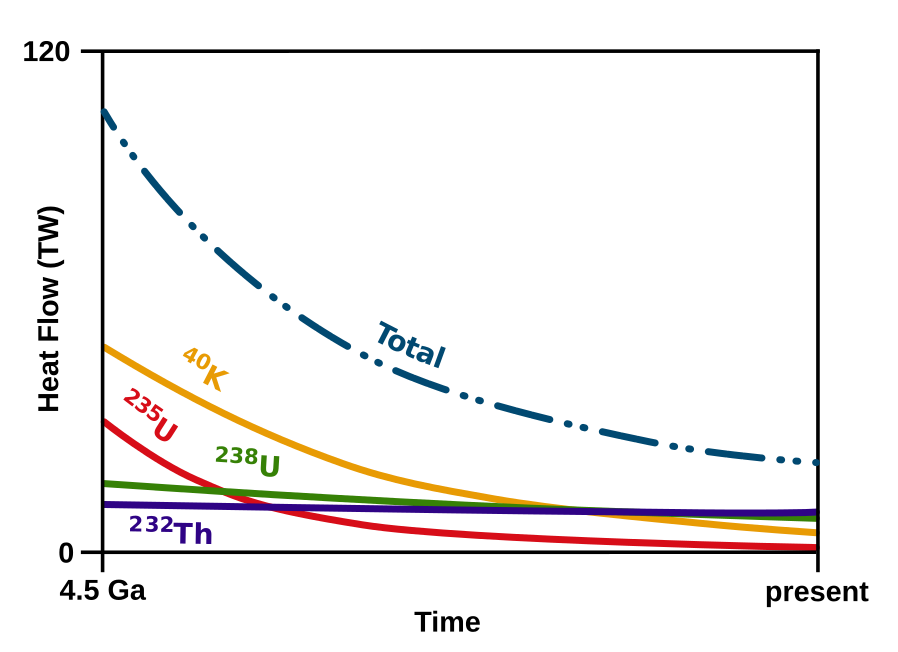
\includegraphics[width=0.95\paperwidth, height=0.70\paperheight, keepaspectratio]{radiogenic_heat_evolution}}\\
  {\footnotesize Two heating clocks: ${}^{26}$Al (dashed) starts near $10^{-7}$ W\,kg$^{-1}$ and dies within about 10 Myr; ${}^{60}$Fe is three orders of magnitude weaker; the four long-lived isotopes (solid) give 92 TW at formation and 19 TW today when integrated over the bulk silicate Earth, a factor 4.7. The crossover near 10 Myr hands the heating from planetesimals to planets. Course figure.}
\end{frame}




% ── Short-lived isotopes ──────────────────────────────────
\begin{frame}{Short-lived isotopes: ${}^{26}\mathrm{Al}$}
  \begin{itemize}
    \item Half-life: only 0.72~Myr (now extinct)
    \item Produced by nearby stellar nucleosynthesis, delivered into the protoplanetary disk
    \item Initial ${}^{26}\mathrm{Al}/^{27}\mathrm{Al}$ ratio $\sim 5 \times 10^{-5}$ (canonical)
    \item In the first few Myr: extraordinarily potent heat source ($10^{-7}$~W\,kg$^{-1}$ initially)
    \item Could melt planetesimals as small as a few km radius
    \item Initiated core formation and volatile loss \textbf{before} planets fully assembled
  \end{itemize}
  \vskip8pt
  \keyresult{${}^{26}\mathrm{Al}$ is why even small asteroids show evidence of melting and differentiation in the meteorite record.}
\end{frame}

\begin{frame}
  \centering
  \makebox[\linewidth][c]{\includegraphics[width=0.95\paperwidth, height=0.63\paperheight, keepaspectratio]{short_lived_decay}}\\
  {\footnotesize Decay of ${}^{26}$Al (half-life 0.72 Myr, daughter ${}^{26}$Mg) and ${}^{60}$Fe (2.6 Myr, ${}^{60}$Ni) over the first 10 Myr. The other extinct clocks, ${}^{53}$Mn--${}^{53}$Cr (3.7 Myr), ${}^{182}$Hf--${}^{182}$W (8.9 Myr), ${}^{129}$I--${}^{129}$Xe (16 Myr) and ${}^{244}$Pu--Xe (81 Myr), date early differentiation, core formation, atmosphere retention and the closure of mantle degassing. ${}^{26}$Al came from a nearby massive star or supernova, so the Sun formed in a massive star cluster. Course figure.}
\end{frame}

% ── Nucleosynthesis origins ──────────────────────────────


% ── 60Fe and other short-lived isotopes ───────────────────


% ── Extinct radionuclide chronometers ──────────────────


% ── Heat budget over time ─────────────────────────────────


% ── Earth's heat budget ──────────────────────────────────
\begin{frame}{Earth's heat budget: 47~TW}
  \centering
  \begin{tabular}{l r}
    \toprule
    \textbf{Source} & \textbf{Contribution} \\
    \midrule
    Radiogenic heating (mantle + crust) & $\sim$20~TW \\
    Primordial (secular cooling)        & $\sim$17~TW \\
    Core cooling and solidification     & $\sim$10~TW \\
    Tidal dissipation (from the Moon)   & $\sim$0.1~TW \\
    \midrule
    \textbf{Total}                      & $\sim$\textbf{47~TW} \\
    \bottomrule
  \end{tabular}
  \vskip15pt
  \begin{itemize}
    \item $\sim$40\% from ongoing radioactive decay; 60\% from primordial heat.
    \item Earth is still cooling.
  \end{itemize}
\end{frame}

% ── Heat budget pie ───────────────────────────────────────
\begin{frame}{Earth's heat budget at a glance}
  \begin{columns}[c]
    \column{\recapfigcolnarrow}
    \ipsrecapfig[0.62\textheight]{earth_heat_budget}
    \column{\recaptextcolwide}
    \small
    \begin{itemize}\setlength\itemsep{1pt}
      \item Radiogenic decay (red, 20 TW) and stored primordial heat (orange, 17 TW) carry most of the 47 TW.
      \item Core cooling and inner-core solidification add 10 TW; lunar tidal dissipation, at 0.1 TW, is invisible at this scale.
      \item The balance shifts over time: 4.5 Gyr ago the radiogenic slice alone was almost 5 times larger.
    \end{itemize}
    \vskip2pt\relax
    \keyresult{Earth today runs roughly 40\% on radioactivity and 60\% on its savings account of primordial heat.}
  \end{columns}
\end{frame}



% ════════════════════════════════════════════════════════════
\sectionimage{earth_interior_cutaway}{Earth's interior. Credit: Wikimedia Commons, CC BY-SA 3.0}
\section{Heat transport mechanisms}
% ════════════════════════════════════════════════════════════

% ── Three mechanisms ──────────────────────────────────────
\begin{frame}{Three ways to move heat}
  \begin{description}[Convection:]
    \item[Conduction:] Heat transferred by molecular and atomic collisions, $\vec{q} = -k\nabla T$ (Fourier's law); slow and diffusive; dominant in lithospheres and small bodies.
    \item[Convection:] Heat transported by bulk fluid motion: hot material rises, cool material sinks; dominant in mantles, outer cores and giant-planet interiors.
    \item[Radiation:] Energy carried by electromagnetic waves, $F = \epsilon\sigma T^4$ (Stefan--Boltzmann); dominant at surfaces, in thin atmospheres and in magma oceans above about 2000 K; solid silicates are opaque in the infrared.
  \end{description}
\end{frame}

\begin{frame}
  \centering
  \makebox[\linewidth][c]{\includegraphics[width=0.95\paperwidth, height=0.70\paperheight, keepaspectratio]{heat_transport_modes}}\\
  {\footnotesize Three ways to move heat: conduction through a material down a temperature gradient without bulk motion, convection by rising hot and sinking cold fluid, radiation by photons from a hot surface. Course schematic.}
\end{frame}

\begin{frame}{Conduction: Fourier's law and the diffusion timescale}
  \begin{columns}[c]
    \column{0.5\textwidth}
    \begin{itemize}\setlength\itemsep{2pt}
      \item Heat flux $\vec{q} = -k\nabla T$
      \item Thermal diffusivity $\kappa = k/(\rho c_p) \approx 10^{-6}$ m$^2$\,s$^{-1}$ for rock
      \item Metals have high $k$ but also high $\rho c_p$; rocks have low $k$ and low $\rho c_p$: similar $\kappa$
    \end{itemize}
    \keyresult{$$\tau_{\mathrm{cond}} \sim \frac{L^2}{\kappa}$$}
    \column{0.5\textwidth}
    \small
    \begin{tabular}{l c c}
      \toprule
      \textbf{Material} & $\boldsymbol{k}$ (W\,m$^{-1}$\,K$^{-1}$) & $\boldsymbol{\kappa}$ (m$^2$\,s$^{-1}$) \\
      \midrule
      Silicate rock & 3--5 & $\sim$10$^{-6}$ \\
      Bridgmanite & 5--10 & $\sim$2$\times 10^{-6}$ \\
      Water ice & 2.2 & 1.1$\times 10^{-6}$ \\
      Iron (solid) & 80 & $\sim$2$\times 10^{-5}$ \\
      Air & 0.025 & $\sim$2$\times 10^{-5}$ \\
      \bottomrule
    \end{tabular}
  \end{columns}
\end{frame}

\begin{frame}
  \centering
  \makebox[\linewidth][c]{\includegraphics[width=0.95\paperwidth, height=0.70\paperheight, keepaspectratio]{fourier_conductivity}}\\
  {\footnotesize Fourier's law in a slab, and the thermal conductivity of planetary materials from air (0.025) to solid iron (80 W\,m$^{-1}$\,K$^{-1}$). Course figure.}
\end{frame}

% ── Conduction details ────────────────────────────────────


% ── Thermal conductivity values ───────────────────────────


% ── Radiation dominance ───────────────────────────────────


% ── Convection overview ──────────────────────────────────
\begin{frame}{Convection: nature's heat elevator}
  \begin{columns}[c]
    \column{\recapfigcolnarrow}
    \centering
    \ipsrecapfig{convection_cells}
    \source{Wikimedia Commons, CC BY-SA 3.0}

    \column{\recaptextcolwide}
    \begin{itemize}
      \item Hot material at base: buoyant, rises
      \item Cool material at top: dense, sinks
      \item Far more efficient than conduction
      \item Active in:
      \begin{itemize}
        \item Earth's mantle ($\sim$cm/yr)
        \item Outer core (liquid metal)
        \item Giant planet interiors
        \item Atmospheres
      \end{itemize}
    \end{itemize}
  \end{columns}
\end{frame}

% ── Rayleigh-Benard schematic pair ────────────────────────
\begin{frame}
  \centering
  \makebox[\linewidth][c]{\includegraphics[width=0.95\paperwidth, height=0.70\paperheight, keepaspectratio]{rayleigh_benard_schematic}}\\
  {\footnotesize Rayleigh-B\'enard convection: hot plumes rise from a thin basal boundary layer, cold fluid sinks from the top one, and lateral flow closes the cells. Convection switches on once Ra exceeds $\mathrm{Ra}_c$. Thin conductive skins around a well-mixed interior: that is mantle convection in one sketch. Course schematic.}
\end{frame}





% ════════════════════════════════════════════════════════════
\sectionimage{earth_interior_cutaway}{Earth's interior. Credit: Wikimedia Commons, CC BY-SA 3.0}
\section{Blackboard derivation: cooling timescale}
% ════════════════════════════════════════════════════════════

% ── Setup: goal and strategy ──────────────────────────────
\begin{frame}{Goal and strategy}
  \textbf{Goal:} Estimate how long it takes heat to conduct out of a body of size $L$.
  \vskip8pt
  \textbf{Strategy:} Start from the heat equation, then use dimensional analysis instead of solving the PDE.
  \vskip10pt
  \begin{itemize}
    \item We want a characteristic timescale $\tau_{\mathrm{cond}}(L, \kappa)$
    \item Plug in representative values for rock
    \item Compare to the age of the solar system ($4.6$~Gyr)
  \end{itemize}
  \vskip8pt
  \textbf{Physical intuition:} bigger bodies have a longer path for heat to diffuse, so they stay hot for longer. We will derive exactly \textit{how much} longer.
\end{frame}

% ── Step 1: heat equation ─────────────────────────────────
\begin{frame}{Step 1: the heat diffusion equation}
  Fourier's law $\vec{q} = -k\nabla T$ combined with energy conservation gives:
  $$\rho c_p\,\pdv{T}{t} = \nabla\!\cdot\!(k\nabla T)$$
  \vskip6pt
  For constant thermal conductivity $k$, define $\kappa = k/(\rho c_p)$:
  $$\pdv{T}{t} = \kappa \nabla^2 T$$
  \vskip6pt
  In one dimension:
  $$\pdv{T}{t} = \kappa \pdv{^2 T}{x^2}$$
  \vskip6pt
  The rate of temperature change is proportional to the \textbf{curvature} of the temperature profile; flat profiles do not evolve, curved ones relax.
\end{frame}

% ── Step 2: dimensional analysis ──────────────────────────
\begin{frame}{Step 2: dimensional analysis}
  Replace derivatives with characteristic scales:
  \begin{itemize}\setlength\itemsep{1pt}
    \item Time derivative: $\pdv{T}{t} \sim \dfrac{T}{\tau}$
    \item Spatial derivative: $\pdv{^2 T}{x^2} \sim \dfrac{T}{L^2}$
  \end{itemize}
  Substitute into the heat equation:
  $$\frac{T}{\tau} \sim \kappa\,\frac{T}{L^2}$$
  \vskip2pt
  Temperature cancels: the timescale is intrinsic, not tied to any particular $T$.
  \vskip2pt
  \keyresult{$$\boxed{\tau_{\mathrm{cond}} \sim \frac{L^2}{\kappa}}$$}
  \vskip4pt
  \textbf{Key feature:} the $L^2$ scaling. Doubling the body size $\rightarrow$ 4$\times$ the cooling time.
\end{frame}

% ── Application table ──────────────────────────────────────
\begin{frame}{Cooling timescales across the solar system}
  Using $\kappa \approx 10^{-6}$~m$^2$\,s$^{-1}$ (silicate rock):
  \vskip8pt
  \centering
  \begin{tabular}{l r r r}
    \toprule
    \textbf{Body} & \textbf{Size $L$} & $\boldsymbol{\tau = L^2/\kappa}$ & \textbf{Familiar units} \\
    \midrule
    1~m boulder  & 1~m               & $10^6$~s              & $\sim$12 days \\
    100~km asteroid & $10^5$~m        & $10^{16}$~s           & $\sim$300~Myr \\
    Moon         & $1.7 \times 10^6$~m & $3 \times 10^{18}$~s & $\sim$100~Gyr \\
    Earth        & $6.4 \times 10^6$~m & $4 \times 10^{19}$~s & $\sim$1300~Gyr \\
    \bottomrule
  \end{tabular}
  \vskip10pt
  \begin{alertblock}{}
    Earth's conductive cooling time $\gg$ age of the universe.\\
    Yet Earth loses 47~TW $\Rightarrow$ there \textbf{must} be convection.
  \end{alertblock}
\end{frame}

% ── tau_cond pair ─────────────────────────────────────────
\begin{frame}
  \centering
  \makebox[\linewidth][c]{\includegraphics[width=0.95\paperwidth, height=0.70\paperheight, keepaspectratio]{tau_cond_vs_size}}\\
  {\footnotesize The conductive cooling time $\tau = L^2/\kappa$ against body size (slope 2 on log axes): a 0.5 mm chondrule cools in under a second, a 1 km asteroid in about 30\,000 yr; the Moon, Mars and Earth would need longer than the age of the universe. Any body larger than a few hundred km must convect, or stay hot. Course figure.}
\end{frame}



% ── Half-space cooling pair ───────────────────────────────
\begin{frame}
  \centering
  \makebox[\linewidth][c]{\includegraphics[width=0.95\paperwidth, height=0.70\paperheight, keepaspectratio]{half_space_cooling}}\\
  {\footnotesize Half-space cooling: each curve is the error-function solution $T(z,t) = T_s + (T_m - T_s)\,\mathrm{erf}\!\big(z/2\sqrt{\kappa t}\big)$ for ages 1 to 200 Myr. The lithosphere thickens as $\sqrt{\kappa t}$, the heat flux falls as $t^{-1/2}$, and the seafloor deepens with age: one solution explains lithosphere thickness, seafloor heat flow and bathymetry. Course figure, after Turcotte \& Schubert (2002).}
\end{frame}





% ── Break ───────────────────────────────────────────────────
\breakslide

% ════════════════════════════════════════════════════════════
\sectionimage{earth_interior_cutaway}{Earth's interior. Credit: Wikimedia Commons, CC BY-SA 3.0}
\section{Rayleigh number \& convective vigour}
% ════════════════════════════════════════════════════════════

% ── Rayleigh number ───────────────────────────────────────
\begin{frame}{The Rayleigh number}
  Does a fluid layer convect or merely conduct?
  \vskip8pt
  $$\mathrm{Ra} = \frac{\alpha \rho g \Delta T\, d^3}{\kappa \eta}$$
  \vskip6pt
  \begin{columns}[T]
    \column{0.48\textwidth}
    \textbf{Numerator} (buoyancy):
    \begin{itemize}
      \item $\alpha$ = thermal expansion
      \item $\rho$ = density
      \item $g$ = gravity
      \item $\Delta T$ = temperature contrast
      \item $d$ = layer depth
    \end{itemize}

    \column{0.48\textwidth}
    \textbf{Denominator} (dissipation):
    \begin{itemize}
      \item $\kappa$ = thermal diffusivity
      \item $\eta$ = dynamic viscosity
    \end{itemize}
    \vskip10pt
    Critical value: $\mathrm{Ra}_c \approx 1708$\\
    {\small (rigid boundaries: fluid sticks to wall; $658$ for free-slip: fluid slides without friction)}
  \end{columns}
\end{frame}

% ── Marginal stability pair ───────────────────────────────
\begin{frame}
  \centering
  \makebox[\linewidth][c]{\includegraphics[width=0.95\paperwidth, height=0.70\paperheight, keepaspectratio]{marginal_stability}}\\
  {\footnotesize Marginal stability: below the curve every perturbation decays and conduction is the only steady state; above it convection grows. The minimum is $\mathrm{Ra}_c \approx 1708$ at wavenumber $k_c \approx 3.12$: convection is a threshold with a preferred cell size set by the layer depth. Course figure, after Turcotte \& Schubert (2002).}
\end{frame}




% ── Earth's mantle Ra ─────────────────────────────────────
\begin{frame}{Earth's mantle: vigorous convection, and how efficient}
  $$\mathrm{Ra}_\oplus \sim \frac{2 \times 10^{-5} \times 4000 \times 10 \times 2500 \times (3 \times 10^6)^3}{10^{-6} \times 10^{21}} \sim 10^7\text{--}10^8 \gg \mathrm{Ra}_c \approx 1708$$
  \begin{itemize}\setlength\itemsep{2pt}
    \item The Nusselt number $\mathrm{Nu} = q_{\mathrm{total}}/q_{\mathrm{cond}}$ measures the efficiency: $\mathrm{Nu} = 1$ is pure conduction.
    \item Boundary-layer theory gives $\mathrm{Nu} \propto \mathrm{Ra}^{1/3}$: doubling Ra adds only about 26\%; a factor $10^3$ in Ra gives a factor 10 in Nu.
  \end{itemize}
  \keyresult{For Earth, $\mathrm{Nu} = (\mathrm{Ra}/\mathrm{Ra}_c)^{1/3} \approx 18$--$39$: convection moves heat tens of times faster than conduction, and the interior cools efficiently.}
  \sourcenote{Schubert et al.\ (2001), \textit{Mantle Convection in the Earth and Planets}}
\end{frame}

% ── Rayleigh number comparison ────────────────────────────
\begin{frame}{Rayleigh number across the solar system}
  \centering
  \small
  \begin{tabular}{l c l}
    \toprule
    \textbf{Body} & \textbf{Ra} & \textbf{Regime} \\
    \midrule
    Earth's mantle      & $10^7$--$10^8$ & Vigorous convection \\
    Venus' mantle       & $10^7$--$10^8$ & Vigorous (stagnant lid) \\
    Mars' mantle        & $10^6$--$10^7$ & Moderate convection \\
    Moon's mantle       & $10^4$--$10^5$ & Weak; cooling by conduction \\
    Mercury's mantle    & $\sim$$10^4$    & Marginal; largely cooled \\
    Magma ocean         & $\gtrsim 10^{25}$ & Turbulent convection \\
    Earth's outer core  & $\gtrsim 10^{25}$ & Turbulent (dynamo) \\
    \bottomrule
  \end{tabular}
  \vskip6pt
  \flushleft
  {\small Ra is hyper-sensitive to size ($\propto d^3$) and viscosity ($\propto 1/\eta$). Small bodies and very viscous interiors quickly drop below Ra$_c$.}
\end{frame}

% ── Nusselt scaling ───────────────────────────────────────


% ── Nu-Ra pair ────────────────────────────────────────────
\begin{frame}
  \centering
  \makebox[\linewidth][c]{\includegraphics[width=0.95\paperwidth, height=0.70\paperheight, keepaspectratio]{nu_ra_scaling}}\\
  {\footnotesize $\mathrm{Nu} = 1$ below $\mathrm{Ra}_c$; above it $\mathrm{Nu} \propto \mathrm{Ra}^{1/3}$. Earth's mantle at $\mathrm{Ra} \sim 10^7$ to $10^8$ (shaded) moves heat 18 to 39 times faster than conduction, but the weak 1/3 power means the efficiency grows only gently with the driving: even vigorous mantles need Gyr to cool. Course figure.}
\end{frame}




% ── Boundary layers ───────────────────────────────────────
\begin{frame}{Thermal boundary layers}
  A convecting interior develops three layers:
  \vskip6pt
  \begin{enumerate}
    \item \textbf{Cold boundary layer (top):} conductive, steep $T$ drop\\
    $\rightarrow$ Earth's \textbf{lithosphere} ($\sim$100--200~km)
    \vskip4pt
    \item \textbf{Well-mixed interior:} nearly adiabatic, slow $T$ variation\\
    $\rightarrow$ bulk of the mantle
    \vskip4pt
    \item \textbf{Hot boundary layer (bottom):} steep $T$ rise into the core\\
    $\rightarrow$ Earth's \textbf{D'' layer} (pronounced ``D double prime''; $\sim$200~km)
  \end{enumerate}
  \vskip8pt
  Nearly all the temperature drop occurs in the two thin boundary layers.
\end{frame}

% ── Adiabatic temperature gradient ───────────────────────
\begin{frame}{The adiabatic gradient}
  In the well-mixed convecting interior, temperature follows an \textbf{adiabat}:
  \vskip6pt
  $$\left(\dv{T}{r}\right)_{\mathrm{adiabat}} = -\frac{\alpha g T}{c_p}$$
  \vskip6pt
  \begin{itemize}
    \item $\alpha$ = thermal expansion, $g$ = gravity, $c_p$ = specific heat
    \item For Earth's upper mantle: $\sim$0.3--0.5~K/km (a fraction of a K per km)
    \item Much shallower than the conductive gradient in the lithosphere ($\sim$25~K/km)
    \item Adiabatic profiles are nearly isothermal on the scale of the mantle
  \end{itemize}
  \vskip6pt
  \keyresult{Temperature changes only a few hundred K over the entire convecting mantle: efficient mixing keeps the interior nearly adiabatic.}
\end{frame}

% ── Mantle adiabat pair ───────────────────────────────────
\begin{frame}
  \centering
  \makebox[\linewidth][c]{\includegraphics[width=0.95\paperwidth, height=0.70\paperheight, keepaspectratio]{mantle_adiabat_tbl}}\\
  {\footnotesize Earth's mantle temperature: a cold boundary layer (the lithosphere, about 100 km) with a steep conductive gradient, a near-adiabatic interior at about 0.5 K\,km$^{-1}$, and the hot D$''$ layer (about 200 km) that bridges the 2500 K adiabat to the 4000 K core-mantle boundary. Almost the whole temperature drop sits in two thin skins. Schematic after Schubert et al.\ (2001).}
\end{frame}




% ── Tectonic regimes ──────────────────────────────────────
\begin{frame}{Two tectonic regimes}
  \begin{columns}[c]
    \column{\recaptextcolwide}
    \small
    \textbf{Mobile lid (plate tectonics):}
    \begin{itemize}\setlength\itemsep{0pt}
      \item Cold boundary layer \textbf{breaks} into plates
      \item Plates subduct, recycle material
      \item Most efficient heat loss
      \item \textbf{Only Earth}
    \end{itemize}
    \textbf{Stagnant lid:}
    \begin{itemize}\setlength\itemsep{0pt}
      \item Single thick, immobile shell
      \item Heat escapes by conduction + volcanism
      \item Less efficient cooling
      \item Venus, Mars, Mercury, Moon
    \end{itemize}
    \vspace{-3pt}
    Why only Earth: likely water, size, and thermal history together.

    \column{\recapfigcolnarrow}
    \centering
    \ipsrecapfig[0.66\textheight]{stern2018_tectonic_stages}
    \source{Reproduced from Stern et al.\ (2018), Fig.~3}
  \end{columns}
\end{frame}

% ── Tectonic modes pair ───────────────────────────────────
\begin{frame}
  \centering
  \makebox[\linewidth][c]{\includegraphics[width=0.95\paperwidth, height=0.70\paperheight, keepaspectratio]{lenardic2018_tectonic_modes}}\\
  {\footnotesize The taxonomy of tectonic modes: active lids (plate tectonics, ridge-only, distributed deformation), episodic modes, and stagnant lids in cold and hot (heat-pipe, plume-fed) variants. Mobile and stagnant are the two end-members of a spectrum that a planet can move through as it cools. Reproduced from Lenardic (2018), Fig.~2.}
\end{frame}

\begin{frame}
  \centering
  \makebox[\linewidth][c]{\includegraphics[width=0.95\paperwidth, height=0.70\paperheight, keepaspectratio]{lyu2025_tectonic_regimes}}\\
  {\footnotesize Six tectonic lid regimes in numerical mantle convection simulations (temperature left, basalt fraction right in each annulus): mobile, stagnant, episodic, sluggish, plutonic-squishy and episodic-squishy lid. Reproduced from Lyu et al.\ (2025), Fig.~1, CC BY 4.0.}
\end{frame}



% ── Plate boundaries cross-section pair ───────────────────
\begin{frame}
  \centering
  \makebox[\linewidth][c]{\includegraphics[width=0.95\paperwidth, height=0.70\paperheight, keepaspectratio]{usgs_plate_boundaries_cross_section}}\\
  {\footnotesize The plate-tectonic settings in one cross-section: ridges where mantle upwells and new crust forms, convergent margins where the cold plate subducts and feeds arc volcanism, and a plume rising independently of the plates. The lithosphere is the cold thermal boundary layer of mantle convection, and subduction is its cold downwelling. Credit: USGS, public domain.}
\end{frame}




% ── Why Earth has plate tectonics ────────────────────────
\begin{frame}{Why does Earth have plate tectonics?}
  \begin{columns}[c]
    \column{\recaptextcolwide}
    \footnotesize
    One of the biggest open questions in planetary geophysics. Proposed factors:
    \begin{itemize}\setlength\itemsep{1pt}
      \item \textbf{Water:} weakens faults; lowers the melting point in subducting slabs
      \item \textbf{Planet size:} higher convective stresses in a larger mantle
      \item \textbf{Thermal state:} cold enough for a rigid lid, hot enough for rifting
      \item \textbf{Prior history:} once started, recycling weakens the lid; may be self-sustaining
      \item Venus: deformed tessera terrain records past plate tectonics, lost after drying out
    \end{itemize}

    \column{\recapfigcolnarrow}
    \centering
    \ipsrecapfig{lyu2025_regime_map}
    \source{Simulated tectonic regimes vs.\ lithosphere strength and internal heating; reproduced from Lyu et al.\ (2025), Fig.~5b, CC BY 4.0}
  \end{columns}
  \vskip2pt
  \keyresult{Habitability-oriented view: plate tectonics is linked to liquid water, and both are linked to long-term climate stability.}
\end{frame}

% ── Heat-pipe volcanism ──────────────────────────────────
\begin{frame}{Heat-pipe volcanism}
  An alternative heat-loss regime for very hot bodies.
  \vskip4pt
  \begin{columns}[c]
    \column{\recaptextcolwide}
    \small
    \begin{itemize}\setlength\itemsep{1pt}
      \item Magma rises through conduits (``heat pipes'')
      \item Erupts on the surface, cools, and is buried by new lava
      \item Old crust subsides into the hot interior as new lava covers it
      \item \textbf{Io today:} global resurfacing by volcanism every $\sim$10$^6$~yr
      \item \textbf{Early Earth:} may have been a heat-pipe regime (Hadean, $>$4~Ga)
      \item Allows efficient cooling of a very hot mantle without plate tectonics
    \end{itemize}

    \column{\recapfigcolnarrow}
    \centering
    \ipsrecapfig{heat_pipe}
    \source{Custom schematic, after Moore \& Webb (2013)}
  \end{columns}
  \vskip2pt
  \sourcenote{Turcotte (1989); Moore \& Webb (2013), \textit{Nature}}
\end{frame}

\begin{frame}
  \centering
  \makebox[\linewidth][c]{\includegraphics[width=0.95\paperwidth, height=0.70\paperheight, keepaspectratio]{tectonic_heat_loss}}\\
  {\footnotesize Heat loss under three regimes: a mobile lid loses heat at ridges and subduction zones, a stagnant lid only by conduction through a thick lid plus episodic volcanism, a heat pipe by erupting and burying magma, as on Io. Course schematic.}
\end{frame}

% ── Mantle plumes and hotspots ────────────────────────────
\begin{frame}{Mantle plumes and hotspots}
  Whole-mantle convection is dominated by sheet-like downwellings (subducting slabs), but the hot bottom boundary layer is also unstable.
  \vskip6pt
  \begin{itemize}
    \item Hot, buoyant material collects at the base of the mantle (D$''$)
    \item Periodically detaches as narrow, rising \textbf{plumes} ($\sim$100~km diameter)
    \item Reach the lithosphere and generate \textbf{intraplate volcanism}
    \item Plumes are long-lived ($10^7$--$10^8$~yr) and approximately fixed in the deep mantle
  \end{itemize}
  \vskip6pt
  \textbf{Examples (Earth):} Hawaii, Iceland, Yellowstone, Réunion.
  \vskip6pt
  \keyresult{Plumes move heat from the core--mantle boundary to the surface independently of plate tectonics.}
\end{frame}

% ── Hotspots map pair ─────────────────────────────────────
\begin{frame}
  \centering
  \makebox[\linewidth][c]{\includegraphics[width=0.95\paperwidth, height=0.70\paperheight, keepaspectratio]{usgs_global_hotspots_map}}\\
  {\footnotesize Plate boundaries and hotspots: hotspots sit on ridges (Iceland, Azores) and inside plates (Hawaii, Yellowstone). Intraplate hotspots are the surface expression of plumes rooted near the core-mantle boundary, fixed while the plates drift over them, so hotspot chains record plate motion over the deep mantle. Credit: USGS, public domain.}
\end{frame}





% ════════════════════════════════════════════════════════════
\sectionimage{enceladus_plumes}{Enceladus plumes, Cassini. Credit: NASA/JPL/SSI}
\section{Surface heat flow \& tidal heating}
% ════════════════════════════════════════════════════════════

% ── Core cooling and the dynamo ──────────────────────────
\begin{frame}{Core cooling and the dynamo}
  The mantle acts as a thermostat on the core.
  \vskip6pt
  \begin{itemize}
    \item Heat flux from core to mantle sets the rate of core cooling
    \item A vigorously convecting mantle extracts heat efficiently, enabling core convection
    \item Core cooling drives the inner core's gradual crystallisation
    \item Inner core growth releases latent heat + light elements $\rightarrow$ compositional buoyancy
    \item This compositional convection is the \textbf{dominant} driver of today's geodynamo (Lecture~4)
  \end{itemize}
  \vskip6pt
  \keyresult{Earth's magnetic field ultimately exists because mantle convection efficiently cools the core; stagnant-lid Venus likely lacks this.}
\end{frame}

% ── Whole-mantle vs layered convection ──────────────────
\begin{frame}{Whole-mantle vs.\ layered convection}
  \textbf{The debate:} does Earth's mantle convect as one layer or two?
  \vskip2pt
  \centering
  \makebox[\linewidth][c]{\includegraphics[width=0.72\linewidth, height=0.41\textheight, keepaspectratio]{whole_vs_layered_convection}}
  \vskip2pt
  \small
  \begin{itemize}\setlength\itemsep{1pt}
    \item Seismic tomography (3-D imaging with earthquake waves) shows the Farallon slab, an ancient subducted plate, sinking to the core--mantle boundary, with plumes rooted at its base
    \item Strong evidence for \textbf{whole-mantle convection}: the 660~km boundary slows slabs but does not stop them
  \end{itemize}
  \vskip2pt
  {\tiny\color{ipsText!60} Custom schematic; tomographic evidence: Grand (2002); Ritsema et al.\ (2011)}
\end{frame}

% ── Mantle plume detail ──────────────────────────────────
\begin{frame}{Plumes vs.\ plates: two modes of upwelling}
  \centering
  \makebox[\linewidth][c]{\includegraphics[width=0.80\linewidth, height=0.36\textheight, keepaspectratio]{plume_vs_ridge_upwelling}}
  \vskip2pt
  \small
  \begin{itemize}\setlength\itemsep{1pt}
    \item \textbf{Mid-ocean ridges:} passive upwelling where plates pull apart; temperatures close to the ambient mantle
    \item \textbf{Mantle plumes:} active upwelling from the deep mantle, $\sim$200 to 300~K hotter; they carry primordial ($^3$He-rich) material from the lower mantle
    \item \textbf{Large Igneous Provinces (LIPs)}, regions covered by exceptionally voluminous basalt eruptions, may be plume-heads (Deccan Traps, Siberian Traps, Ontong-Java Plateau); LIPs correlate with mass extinctions
  \end{itemize}
  \vskip2pt
  {\tiny\color{ipsText!60} Custom schematic; source: Courtillot \& Renne (2003), \textit{Comptes Rendus Geoscience}}
\end{frame}


% ── Surface heat flow ─────────────────────────────────────
\begin{frame}{Surface heat flow}
  \centering
  \begin{tabular}{l c c l}
    \toprule
    \textbf{Body} & \textbf{Heat flux (mW\,m$^{-2}$)} & \textbf{Total (TW)} & \textbf{Source} \\
    \midrule
    Earth  & $\sim$90   & $\sim$47   & Radiogenic + primordial \\
    Moon   & 10--15     & $\sim$0.3  & Primordial (cooled) \\
    Mars   & 15--25     & $\sim$2--4 & Radiogenic + primordial \\
    Io     & 2000--2500 & $\sim$105 & \textbf{Tidal dissipation} \\
    \bottomrule
  \end{tabular}
  \vskip6pt
  \sourcenote{Davies \& Davies (2010); Davies et al.\ (2024); InSight + gravity/topography estimates}
  \vskip10pt
  Earth's 47 TW leave 70\% through the oceans (60\% of the area) and 30\% through the continents, where about 40\% of the surface flux is crustal-radiogenic.\\[3pt]
  Io's heat flux is 20--30$\times$ higher than Earth's per unit area, and its total power ($105 \pm 12$~TW) is roughly \textbf{twice} Earth's 47~TW, from a body with only 1.5\% of Earth's mass.
\end{frame}

% ── Earth heat flow spatial pattern ──────────────────────


% ── Heat flow map pair ────────────────────────────────────
\begin{frame}
  \centering
  \makebox[\linewidth][c]{\includegraphics[width=0.95\paperwidth, height=0.66\paperheight, keepaspectratio]{earth_heat_flow_map}}\\
  {\footnotesize Surface heat flow: mid-ocean ridges are the hottest features, heat flow falls with seafloor age as the half-space model predicts, and old continental shields are the coldest surfaces. The compilation behind the map holds about 70\,000 measurements; Earth's total heat loss is 47 TW (Davies \& Davies 2010). Plate tectonics made visible in one quantity. Credit: Fabio Crameri (Wikimedia, CC BY-SA 4.0); data from Lucazeau (2019).}
\end{frame}



% ── q vs age pair ─────────────────────────────────────────
\begin{frame}
  \centering
  \makebox[\linewidth][c]{\includegraphics[width=0.95\paperwidth, height=0.66\paperheight, keepaspectratio]{q_vs_seafloor_age}}\\
  {\footnotesize Seafloor heat flux against crustal age: the half-space prediction $q \propto t^{-1/2}$ (blue) against measurements in 2.5 Myr bins filtered for hydrothermal sites (grey). Raw young-crust surveys fall below the curve because hydrothermal circulation carries part of the heat; old crust reaches the plate-cooling asymptote near 48 mW\,m$^{-2}$. Data: Richards et al.\ (2018); asymptote after Stein \& Stein (1992).}
\end{frame}




% ── Secular cooling ──────────────────────────────────────
\begin{frame}{Secular cooling of planets}
  Planets are thermally non-stationary: they started hot and are gradually cooling.
  \vskip6pt
  \begin{itemize}
    \item Stored heat $\sim E_{\mathrm{acc}} + E_{\mathrm{diff}} + \int L_{\mathrm{rad}}(t)\,dt$
    \item Lost heat $\sim \int L_{\mathrm{surface}}(t)\,dt$
    \item The difference is the present-day thermal state
    \item Earth: still cooling at $\sim$50--100~K/Gyr
    \item Smaller bodies cool faster (lower thermal inertia, thinner conductive boundary layer)
  \end{itemize}
  \vskip6pt
  \keyresult{All terrestrial planets are in net secular cooling; Earth's is slowed by convective resurfacing but not stopped.}
\end{frame}

% ── Tidal heating mechanism ───────────────────────────────


% ── Tidal heating rate formula ────────────────────────────
\begin{frame}{Tidal heating: eccentric orbits and the dissipation rate}
  \keyresult{$$\dot{E}_{\mathrm{tidal}} = \frac{21}{2}\,\frac{k_2}{Q}\,\frac{G M_p^2 R^5 n e^2}{a^6}$$}
  \begin{itemize}\setlength\itemsep{2pt}
    \item A circular orbit with a tidal lock gives a static bulge and no heating; an eccentric orbit varies the distance, so the deformation flexes each orbit and friction turns it into heat.
    \item $k_2$ is the Love number (about 0.3 for rocky bodies), $Q$ the tidal quality factor (lower means more dissipative), $M_p$ the mass of the primary, $R$ the radius of the moon, $n = \sqrt{GM_p/a^3}$ the mean motion.
    \item Zero $e$ means zero heating; at fixed $e$ the heating scales as $a^{-15/2}$, and the $R^5/a^6$ dependence makes it dramatic for close-in moons.
  \end{itemize}
\end{frame}

% ── Tidal flexing pair ────────────────────────────────────
\begin{frame}
  \centering
  \makebox[\linewidth][c]{\includegraphics[width=0.95\paperwidth, height=0.70\paperheight, keepaspectratio]{tidal_flexing}}\\
  {\footnotesize Tidal flexing on an eccentric orbit: the bulge is largest at periapsis, $r = a(1-e)$, and smallest at apoapsis, $r = a(1+e)$. Each orbit squeezes and stretches the body, and internal friction turns the cyclic work into heat at a rate proportional to $e^2/Q$: no eccentricity, no flexing, no heat. Course schematic.}
\end{frame}




% ── Laplace resonance ─────────────────────────────────────
\begin{frame}{The Laplace resonance: sustaining eccentricity}
  Io's orbit would circularise in $\sim$10~Myr if left alone. Why is its eccentricity maintained?
  \vskip6pt
  \begin{itemize}
    \item Io--Europa--Ganymede are locked in a 4:2:1 \textbf{mean-motion resonance}
    \item Every time Io laps Europa, the two meet at the same orbital phase
    \item Periodic gravitational kicks continually \textbf{pump} Io's eccentricity
    \item Without this, tidal dissipation would damp $e$ and shut off the heating
    \item The resonance was first identified by Laplace in 1805
  \end{itemize}
  \vskip6pt
  \keyresult{The three-body resonance is what makes Io's tidal heating indefinite, not transient.}
\end{frame}

% ── Laplace resonance pair ────────────────────────────────
\begin{frame}
  \centering
  \makebox[\linewidth][c]{\includegraphics[width=0.95\paperwidth, height=0.70\paperheight, keepaspectratio]{laplace_resonance}}\\
  {\footnotesize The Laplace resonance: (a) the three orbits to scale at a Europa-Ganymede conjunction, with Io locked on the opposite side so that a triple conjunction never occurs; (b) periods in the ratio 1:2:4, the pattern repeating every Ganymede orbit. The repeating kicks force Io's eccentricity to about 0.004, small but enough. Course figure.}
\end{frame}




% ── Io ─────────────────────────────────────────────────────
\begin{frame}{Io: the most volcanic body}
  \begin{columns}[c]
    \column{\recapfigcolnarrow}
    \centering
    \ipsrecapfig{io_tvashtar_plume}
    \source{NASA/JHUAPL/SwRI (2007)}

    \column{\recaptextcolwide}
    \begin{itemize}
      \item $\sim 10^{14}$~W of tidal heat (2$\times$ Earth's total!)
      \item Predicted by Peale, Cassen \& Reynolds (1979)
      \item Confirmed days later by Voyager~1
      \item Powered by the \textbf{Laplace resonance}
      \item 343 catalogued active volcanic centres (Davies et al.\ 2024)
      \item Entire surface resurfaced on $\sim$Myr timescale
    \end{itemize}
  \end{columns}
\end{frame}

\begin{frame}
  \centering
  \makebox[\linewidth][c]{\includegraphics[width=0.95\paperwidth, height=0.70\paperheight, keepaspectratio]{io_galileo_color}}\\
  {\footnotesize Io in Galileo colour: volcanic centres, lava flows and yellow-red sulfur deposits cover the globe. 343 active volcanic centres are catalogued, and lava resurfaces the whole moon on a Myr timescale, so Io has essentially no impact craters. Credit: NASA/JPL/University of Arizona, public domain.}
\end{frame}

% ── Io hotspot map pair ───────────────────────────────────
\begin{frame}
  \centering
  \makebox[\linewidth][c]{\includegraphics[width=0.95\paperwidth, height=0.70\paperheight, keepaspectratio]{io_volcanic_heatmap}}\\
  {\footnotesize Io's 343 catalogued hot spots, sized and coloured by power; Loki Patera tops the list at 6000 to 12\,000 GW. Together they emit $58 \pm 1$ TW, about 55\% of Io's $105 \pm 12$ TW; polar volcanoes emit half the energy of lower-latitude ones, which favours shallow over deep-mantle tidal heating. Reproduced from Davies et al.\ (2024), Fig.~1.}
\end{frame}




% ── Enceladus ──────────────────────────────────────────────
\begin{frame}{Enceladus: a tiny moon with a big secret}
  \begin{columns}[c]
    \column{\recapfigcolnarrow}
    \centering
    \ipsrecapfig[0.29\textheight]{enceladus_tiger_stripes_full}
    \vskip4pt
    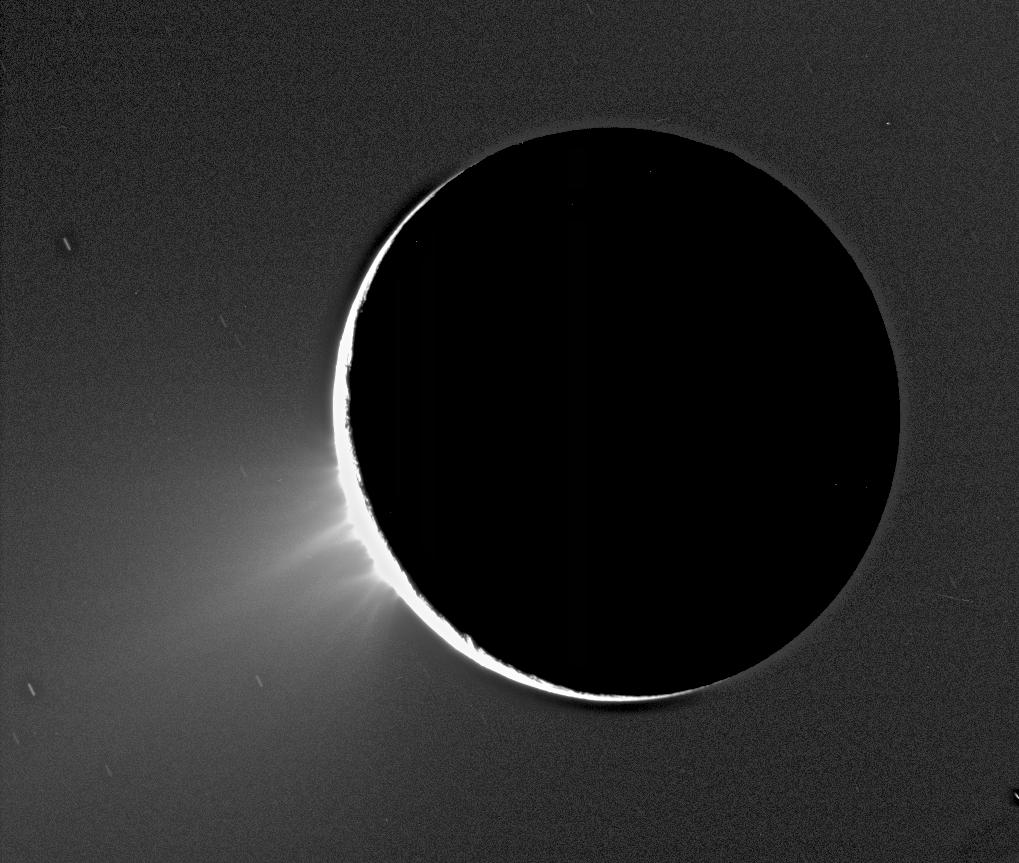
\includegraphics[width=\textwidth,height=0.29\textheight,keepaspectratio]{enceladus_plumes}
    \source{NASA/JPL/SSI (Cassini)}

    \column{\recaptextcolwide}
    \begin{itemize}
      \item Radius only 252~km
      \item Water ice jets from ``tiger stripe'' fractures
      \item Thermal power: $\sim$16~GW (tidal dissipation)
      \item Global subsurface ocean beneath $\sim$15--25~km ice
      \item Plumes carry salts, silica, organics, and $\mathrm{H_2}$: hydrothermal activity on the ocean floor
    \end{itemize}
  \end{columns}
  \vskip2pt
  \keyresult{Tidal heating can sustain liquid-water oceans far outside the habitable zone.}
\end{frame}

% ── Enceladus dissipation location ──────────────────────
\begin{frame}{Where in Enceladus is tidal heat dissipated?}
  Two competing scenarios explain the observed $\sim$16~GW of thermal power:
  \vskip1pt
  \begin{columns}[T]
    \column{0.48\textwidth}
    \textbf{Rocky core dissipation:}
    \begin{itemize}
      \item Tidal flexing of porous silicate core
      \item Heat conducted up through the ocean
      \item Matches hydrothermal signatures (silica nanoparticles at $\sim$90\textdegree C)
      \item Difficulty: plume power exceeds simple core-heating estimates
    \end{itemize}

    \column{0.48\textwidth}
    \textbf{Ice-shell dissipation:}
    \begin{itemize}
      \item Viscous dissipation concentrated in the warm ice shell base
      \item Positive feedback: softer ice $\rightarrow$ more dissipation
      \item Can reach 10--20~GW with realistic ice rheology (deformation behaviour)
      \item Concentrates heat near the south pole tiger stripes
    \end{itemize}
  \end{columns}
  \vskip1pt
  Likely: both contribute, with the ice shell dominating the plume heat flux.
  \vskip1pt
  \sourcenote{\v{C}adek et al.\ (2016); Hemingway \& Mittal (2019)}
\end{frame}

% ── Enceladus thermal scan ────────────────────────────────
\begin{frame}{Where the heat leaves Enceladus}
  \begin{columns}[c]
    \column{\recapfigcolnarrow}
    \ipsrecapfig[0.62\textheight]{enceladus_thermal_map}
    \column{\recaptextcolwide}
    \footnotesize
    \begin{itemize}\setlength\itemsep{1pt}
      \item A high-resolution Cassini CIRS thermal scan (colour) along one tiger-stripe fracture, draped on the visible-light mosaic.
      \item The warm emission hugs the fracture and dies off within a few km to either side: the heat leaves through the cracks, not the plains.
      \item Integrated over the whole south polar terrain: $15.8 \pm 3.1$ GW, far beyond any radiogenic budget for a 252 km moon.
    \end{itemize}
    \vskip2pt\relax
    \keyresult{On Enceladus, tidal heat is not diffuse: it is plumbed to the surface along four fractures.}
  \end{columns}
\end{frame}


% ── Enceladus biosignatures ──────────────────────────────


% ── Ocean worlds ──────────────────────────────────────────
\begin{frame}{Ocean worlds: Enceladus, Europa and Titan}
  \begin{columns}[t]
    \column{0.52\textwidth}
    \textbf{Enceladus plume samples (Cassini):}
    \begin{itemize}\setlength\itemsep{1pt}
      \item Salts (NaCl, NaHCO$_3$): direct samples of the ocean
      \item Silica nanoparticles: ocean floor above 90\textdegree C (hydrothermal)
      \item H$_2$ from water--rock serpentinisation
      \item Organics up to C$_6$; phosphate detected in 2023 (Postberg et al.)
    \end{itemize}
    \column{0.46\textwidth}
    \textbf{Europa:} global ocean about 100 km deep under 15 to 25 km of ice, kept liquid by the Laplace resonance; Europa Clipper (launched 2024).\\[4pt]
    \textbf{Titan:} subsurface water--ammonia ocean, inferred from its rotational state (Cassini); Dragonfly (launch about 2028) explores the surface chemistry.
  \end{columns}
  \vskip4pt
  \keyresult{Liquid water, chemical energy and organic building blocks: the ocean worlds hold all the ingredients for chemoautotrophic life.}
\end{frame}

% ── Europa interior pair ──────────────────────────────────
\begin{frame}
  \centering
  \makebox[\linewidth][c]{\includegraphics[width=0.95\paperwidth, height=0.70\paperheight, keepaspectratio]{europa_interior_cutaway}}\\
  {\footnotesize Europa's interior: an iron-nickel core, a silicate mantle, a global ocean about 100 km deep and an ice shell of 15 to 25 km. Tidal dissipation forced by the Laplace resonance keeps the ocean liquid; Galileo's induction and gravity data are the evidence, and Europa Clipper will measure the shell directly. Credit: NASA/JPL.}
\end{frame}





% ════════════════════════════════════════════════════════════
\sectionimage{io_tvashtar_plume}{Io's Tvashtar plume. Credit: NASA/JHUAPL/SwRI}
\section{Recent advances \& outlook}
% ════════════════════════════════════════════════════════════

% ── Recent advances ───────────────────────────────────────


% ── More recent advances ──────────────────────────────────


% ── InSight pair ──────────────────────────────────────────
\begin{frame}
  \centering
  \makebox[\linewidth][c]{\includegraphics[width=0.95\paperwidth, height=0.70\paperheight, keepaspectratio]{insight_mars_cutaway}}\\
  {\footnotesize InSight: seismic waves from marsquakes and impacts travel along depth-dependent paths, and their arrival times fix the crustal thickness, the mantle structure and the core radius. The 2023 reanalyses add a molten silicate layer of about 150 km above a metal core of about 1675 km. Credit: NASA/JPL-Caltech.}
\end{frame}

\begin{frame}{Modelling Mars' thermal evolution}
  Mars' thermal history explains key observations:
  \vskip6pt
  \begin{itemize}
    \item Early intense volcanism (Tharsis) $\rightarrow$ hot magma ocean + dynamo (4.1~Ga)
    \item Dynamo shutdown $\sim$4.1~Ga $\rightarrow$ core cooling slowed, crustal magnetisation frozen
    \item Olympus Mons still eruptive until $\sim$100--200~Ma
    \item Present-day heat flow $\sim$15--25~mW/m$^2$ (InSight constraints)
    \item Partially molten upper core retains heat; slow mantle convection prolongs cooling
  \end{itemize}
  \vskip6pt
  \keyresult{Mars' thermal history ties directly to its atmospheric evolution: the loss of the dynamo caused the loss of the field, and eventually the atmosphere.}
\end{frame}




% ── Europa Clipper ────────────────────────────────────────


% ── Mars interior heat models ─────────────────────────────


% ── Io heat flow ──────────────────────────────────────────


% ── JUICE ────────────────────────────────────────────────


% ── Ocean world habitability ─────────────────────────────


% ── Summary ────────────────────────────────────────────────
\begin{frame}{The 2030s at the ocean worlds and Io}
  \begin{itemize}\setlength\itemsep{3pt}
    \item \textbf{Europa Clipper} (launched October 2024, at Jupiter in 2030): about 50 flybys; ice-penetrating radar maps the shell thickness, the magnetometer constrains the ocean salinity, and thermal mapping finds thin ice and recent activity. It tests whether tidal dissipation sits in the shell or in the rocky core.
    \item \textbf{JUICE} (launched April 2023, at Jupiter in 2031, in orbit around Ganymede in 2034): ice-shell and ocean thickness from laser altimetry and the induced field, and tidal heating from the Love number $k_2$.
    \item \textbf{Juno at Io} (2021 onwards): a global heat-flow map with hotter poles than simple tidal models predict, and gravity data consistent with a global magma ocean beneath the crust (Park et al.\ 2024).
  \end{itemize}
  \sourcenote{Howell \& Pappalardo (2020); Grasset et al.\ (2013); Park et al.\ (2024)}
\end{frame}

\begin{frame}{Summary}
  \begin{enumerate}
    \item Four heat sources: accretional, gravitational differentiation, radioactive decay, tidal heating
    \item Conduction is diffusive ($\tau \sim L^2/\kappa$), too slow for planet-sized bodies
    \item Convection dominates in large bodies: $\mathrm{Ra} \gg \mathrm{Ra}_c$
    \item Earth: mobile lid (plate tectonics); other rocky bodies: stagnant lid
    \item Tidal heating powers Io's volcanism and maintains subsurface oceans on Enceladus, Europa, and Titan
    \item Earth's total heat loss: 47~TW (40\% radiogenic, 60\% primordial)
  \end{enumerate}
\end{frame}

% ── Looking ahead ───────────────────────────────────────────
\begin{frame}{Looking ahead to Lecture 4}
  This lecture followed the \textbf{heat}: where it comes from and how it escapes.
  \vskip6pt
  Lecture 4 follows the \textbf{chemistry} the heat enables:
  \begin{itemize}
    \item How a molten planet separates into a metallic core and a silicate mantle.
    \item How siderophile and lithophile elements sort themselves between the two.
    \item What the Hf--W chronometer says about how \emph{fast} core formation happened.
    \item How a convecting metallic core generates the magnetic field that shields an atmosphere.
  \end{itemize}
  \vskip6pt
  \keyresult{The heat sources assembled today set the pace for all of it: differentiation needs melting, and the dynamo needs a cooling core.}
\end{frame}

% ── Final slide ─────────────────────────────────────────────
\begin{frame}[plain,noframenumbering]
  \begin{tikzpicture}[remember picture, overlay]
    \ipscontain{title_background}
    \fill[ipsPrimary, opacity=0.70] (current page.north west) rectangle (current page.south east);
  \end{tikzpicture}
  \vfill
  \begin{center}
    {\color{white}\LARGE\bfseries Questions?}\\[14pt]
    {\color{white!85}\large Next: Lecture 4, Chemical differentiation \& magnetospheres}\\[4pt]
    {\color{white!85}\small Thu 17 Sep, 11:00--13:00, room 5419.0161 (Collegezaal)}\\[12pt]
    {\color{white!85}\small Next tutorial: Fri 18 Sep, 13:00--15:00, room 5419.0161 (Collegezaal)}\\[20pt]
    {\color{white!70}\small \texttt{https://ips.formingworlds.space}}
  \end{center}
  \vfill
\end{frame}

\end{document}
